% Optimized XePersian Lab Report Template
% Lightweight, clean, and efficient for bilingual reports with Persian/English text and images

\documentclass[a4paper,12pt]{article}

% --- Essential Packages ---
\usepackage[margin=1in]{geometry}
\usepackage{graphicx}      % for images
\usepackage{caption}       % better captions
\usepackage{subcaption}    % subfigures
\usepackage{float}         % control figure placement
\usepackage{booktabs}      % for tables
\usepackage{hyperref}      % clickable links
\usepackage{xcolor}        % color support
\usepackage{fancyhdr}      % headers and footers
\usepackage{xepersian}     % Persian/English text support

% --- Font Setup ---
\settextfont{IRANSans.ttf}
\settextfont[BoldFont={IRANSans_Medium.ttf}]{IRANSans.ttf}
\setlatintextfont{Times New Roman}
\setlatintextfont[BoldFont={Times New Roman Bold}]{Times New Roman}

% --- Page Style ---
\pagestyle{fancy}
\fancyhf{}
\rhead{\thepage}
\lhead{\lr{CA LAB Report}}
\renewcommand{\headrulewidth}{0.4pt}

% --- Basic Formatting ---
\setlength{\parskip}{0.6em}
\setlength{\parindent}{0pt}
\renewcommand{\figurename}{شکل}
\renewcommand{\tablename}{جدول}
\definecolor{engblue}{RGB}{0, 80, 180}
\definecolor{engred}{RGB}{255, 0, 0}
\definecolor{enggreen}{RGB}{0, 180, 80}
\definecolor{red}{RGB}{180, 0, 0}
\newcommand{\engb}[1]{\textcolor{engblue}{\lr{#1}}}
\newcommand{\engr}[1]{\textcolor{engred}{\lr{#1}}}

% --- Title Page ---
\title{\textbf{\lr{Computer Architecture LAB Report}}}  % Lab Report Title
\author{امیرحسین عالیان \\\lr{4021120017}\\ امیرمهدی عزیزی \\\lr{4021120019}}
\date{}

\begin{document}

\maketitle
\begin{center}
\textbf{آزمایش اول}
\end{center}

\vspace{1cm}
\begin{center}
تاریخ انجام آزمایش: 12 مهر 1404\\
تاریخ تحویل گزارش: 26 مهر 1404
\end{center}
\tableofcontents
\newpage

% ----------------------------
%   Sections
% ----------------------------
\section{چکیده}
\subsection{هدف آزمایش}

هدف این آزمایش، پیاده‌سازی بخشی از مسیر داده (\engb{Datapath}) است که عمدتاً به بخش‌های ارتباطی و گذرگاه (\engb{BUS}) مربوط می‌شود. در این آزمایش، یک گذرگاه دو بیتی و همچنین چهار ثبات (\engb{Register}) دو بیتی طراحی میکنیم.\\
به کمک دو مالتی‌پلکسر چهار‌-به‌-یک (\engb{4-to-1 MUX})، محتوای هر ثباتِ مورد نظر را می‌توان بر روی گذرگاه قرار داد.\\\\
برای اجرای آزمایش، مقادیر ورودی هر ثبات را به‌صورت دلخواه و با استفاده از خطوط \engr{\textbf{V\textsubscript{CC}}} و \lr{\textbf{GND}} تنظیم می‌کنیم. همچنین برای بررسی درستی عملکرد مدار، خروجی گذرگاه را به دو \engb{LED} متصل می‌کنیم (\textcolor{enggreen}{سبز برای بیت پر ارزش} و \textcolor{red}{قرمز برای بیت کم ارزش}) و مقدار \engb{LED} ها را با مقدار ثبات انتخاب شده مقایسه می‌کنیم.
\textbf{}
\subsection{قطعات و ابزار ها}
\begin{latin}
\begin{LTR}
\begin{table}[h!]
	\centering
	\begin{tabular}{llc}
	\toprule
	\textbf{Component} & \textbf{Function} & \textbf{Quantity} \\
	\midrule
IC 74374 & 8-bit Register with 3-state Output & \LR{1} \\
IC 74153 & Dual 4-to-1 Multiplexer & \LR{1} \\
Green LED & MSB Indicator & \LR{1} \\
Red LED & LSB Indicator & \LR{1} \\
Breadboard & Component Placement & \LR{1} \\
DC Power Supply & Provides V\textsubscript{CC} and Common GND & \LR{1} \\
Function Generator & Provides Clock and Common GND & \LR{1} \\
	\bottomrule
	\end{tabular}
	\caption{\rl{لیست قطعات مورد استفاده در این آزمایش}}
	\label{tab:components}
\end{table}
\end{LTR}
\end{latin}

\subsection{پاسخ سوال 1}
\begin{latin}
\begin{LTR}
\begin{table}[h!]
	\centering
	\begin{tabular}{cc}
	\toprule
	\textbf{Select MUX - S\textsubscript{1}S\textsubscript{0}} & \textbf{Output BUS - Y\textsubscript{2}Y\textsubscript{1}} \\
	\midrule
00 & 10 \\
01 & 11 \\
10 & 01 \\
11 & 00 \\
	\bottomrule
	\end{tabular}
	\caption{\rl{جدول مقادیر خروجی}}
	\label{tab:components}
\end{table}
\end{LTR}
\end{latin}

\subsection{پاسخ سوال 2}
در واقع می‌خواهیم خروجی مالتی پلکسر ها را در یک ثبات دو بیتی دیگر ذخیره کنیم، برای اینکار نیاز به یک \engb{IC 74374} دیگر داریم.

\pagebreak
\section{توضیح IC ها}
\subsection{توضیح 74374 IC}
\begin{figure}[H]
    \centering
    \includegraphics[width=0.7\textwidth]{images/74374_Pinouts.jpg}
    \caption{نمایی از پایه های 74374 IC}
    \label{fig:74374}
\end{figure}
\vspace*{0.1cm}
در واقع این \engb{IC} در خود ۸ عدد فلیپ فلاپ (\engb{Flip-Flop}) از نوع \engb{D} دارد. که دارای \engb{Clock} مشترک اند (یک \engb{Register} ۸ بیتی است).\\\\
پایه های \engr{D\textsubscript{i}} به عنوان ورودی های \engb{Register} و پایه های \engr{Q\textsubscript{i}} به عنوان خروجی های \engb{Register} استفاده میشوند.\\\\
باید دقت داشت که خروجی هر یک از فلیپ فلاپ ها به یک بافر ۳ حالته (\engb{3-State Buffer}) متصل است و پایه های \engr{Q\textsubscript{i}} در واقع خروجی های بعد از بافر های ۳ حالته اند.\\\\
خطوط \engb{Enable} این بافر ها همگی به هم دیگر متصل اند و توسط پایه \engr{\lr{$\overline{\mathrm{OC}}$}} کنترل میشوند.\\\\
پایه \engr{\lr{$\overline{\mathrm{OC}}$}} از نوع \engb{Active-Low} است و در صورتی که به آن 1 بدهیم خروجی مدار باز (\engb{High-Impedance}) خواهد بود و در صورتی که به آن 0 بدهیم محتوای فلیپ فلاپ ها روی پایه های \engr{Q\textsubscript{i}} قابل مشاهده خواهند بود.\\

\pagebreak
\subsection{توضیح 74153 IC}
\begin{figure}[H]
    \centering
    \includegraphics[width=0.7\textwidth]{images/74153_Pinouts.jpg}
    \caption{نمایی از پایه های 74153 IC}
    \label{fig:74153}
\end{figure}
\vspace*{1cm}
درون این \engb{IC} دو عدد مالتی‌پلکسر چهار‌-به‌-یک (\engb{4-to-1 MUX}) وجود دارد. (یک مالتی‌پلکسر چهار‌-به‌-یک ۲ بیتی است).\\\\
یکی از این مالتی‌پلکسر ها در سمت چپ \engb{IC} و دیگری در سمت راست آن است.\\\\
به طوری که در سمت چپ پایه های \engr{1C0} تا \engr{1C3} به عنوان 4 بیت ورودی و پایه \engr{ِY1} تک بیت خروجی است.\\
در سمت راست نیز پایه های \engr{2C0} تا \engr{2C3} به عنوان 4 بیت ورودی و پایه \engr{ِY2} تک بیت خروجی است.\\\\
خطوط انتخاب (\engb{Selection Lines}) میان هر دو مالتی‌پلکسر مشترک و به همدیگر متصل است.\\
به طوری که پایه \engr{A} به عنوان خط انتخاب کم ارزش (\engb{S0}) و پایه \engr{B} به عنوان خط انتخاب پر ارزش (\engb{S1}) مورد استفاده قرار می‌گیرد.\\\\
پایه های \engr{\lr{$\overline{\mathrm{1G}}$}} و \engr{\lr{$\overline{\mathrm{2G}}$}} از نوع \engb{Active-Low} هستند و به هر کدام از آنها که 1 بدهیم خروجی آن \engb{MUX} 0 خواهد بود و در صورتی که به هر کدام از آنها 0 بدهیم، خروجی مقدار انتخاب شده از میان ورودی ها خواهد بود که روی پایه های \engr{Y1} و \engr{Y2} قابل مشاهده است.\\


\pagebreak
\section{اتصال قطعات و شماتیک مدار}
\subsection{شکل اولیه}
\begin{figure}[H]
    \centering
    \includegraphics[width=1\textwidth]{images/schematic.pdf}
    \caption{شماتیک مدار در پروتئوس - حالت 4 ثبات}
    \label{fig:schematic}
\end{figure}

\subsection{شکل ثانویه ( پاسخ سوال 3)}
\begin{figure}[H]
    \centering
    \includegraphics[width=1\textwidth]{images/schematic_with_E.pdf}
    \caption{شماتیک مدار در پروتئوس - حالت 5 ثبات}
    \label{fig:schematic}
\end{figure}


\pagebreak
\section{نتایج}
\subsection{نتایج شبیه سازی}
\begin{figure}[H]
    \centering
    \includegraphics[width=1\textwidth]{images/Result1-pr.pdf}
    \caption{خروجی شبیه ساز به ازای \engr{\textbf{S\textsubscript{1}S\textsubscript{0}} = 01}}
    \label{fig:result1}
\end{figure}

\begin{figure}[H]
    \centering
    \includegraphics[width=0.55\textwidth]{images/Result2-pr.pdf}
    \caption{خروجی شبیه ساز به ازای \engr{\textbf{S\textsubscript{1}S\textsubscript{0}} = 11}}
    \label{fig:result2}
\end{figure}

\pagebreak
\subsection{نتایج آزمایش عملی}
\begin{figure}[H]
    \centering
    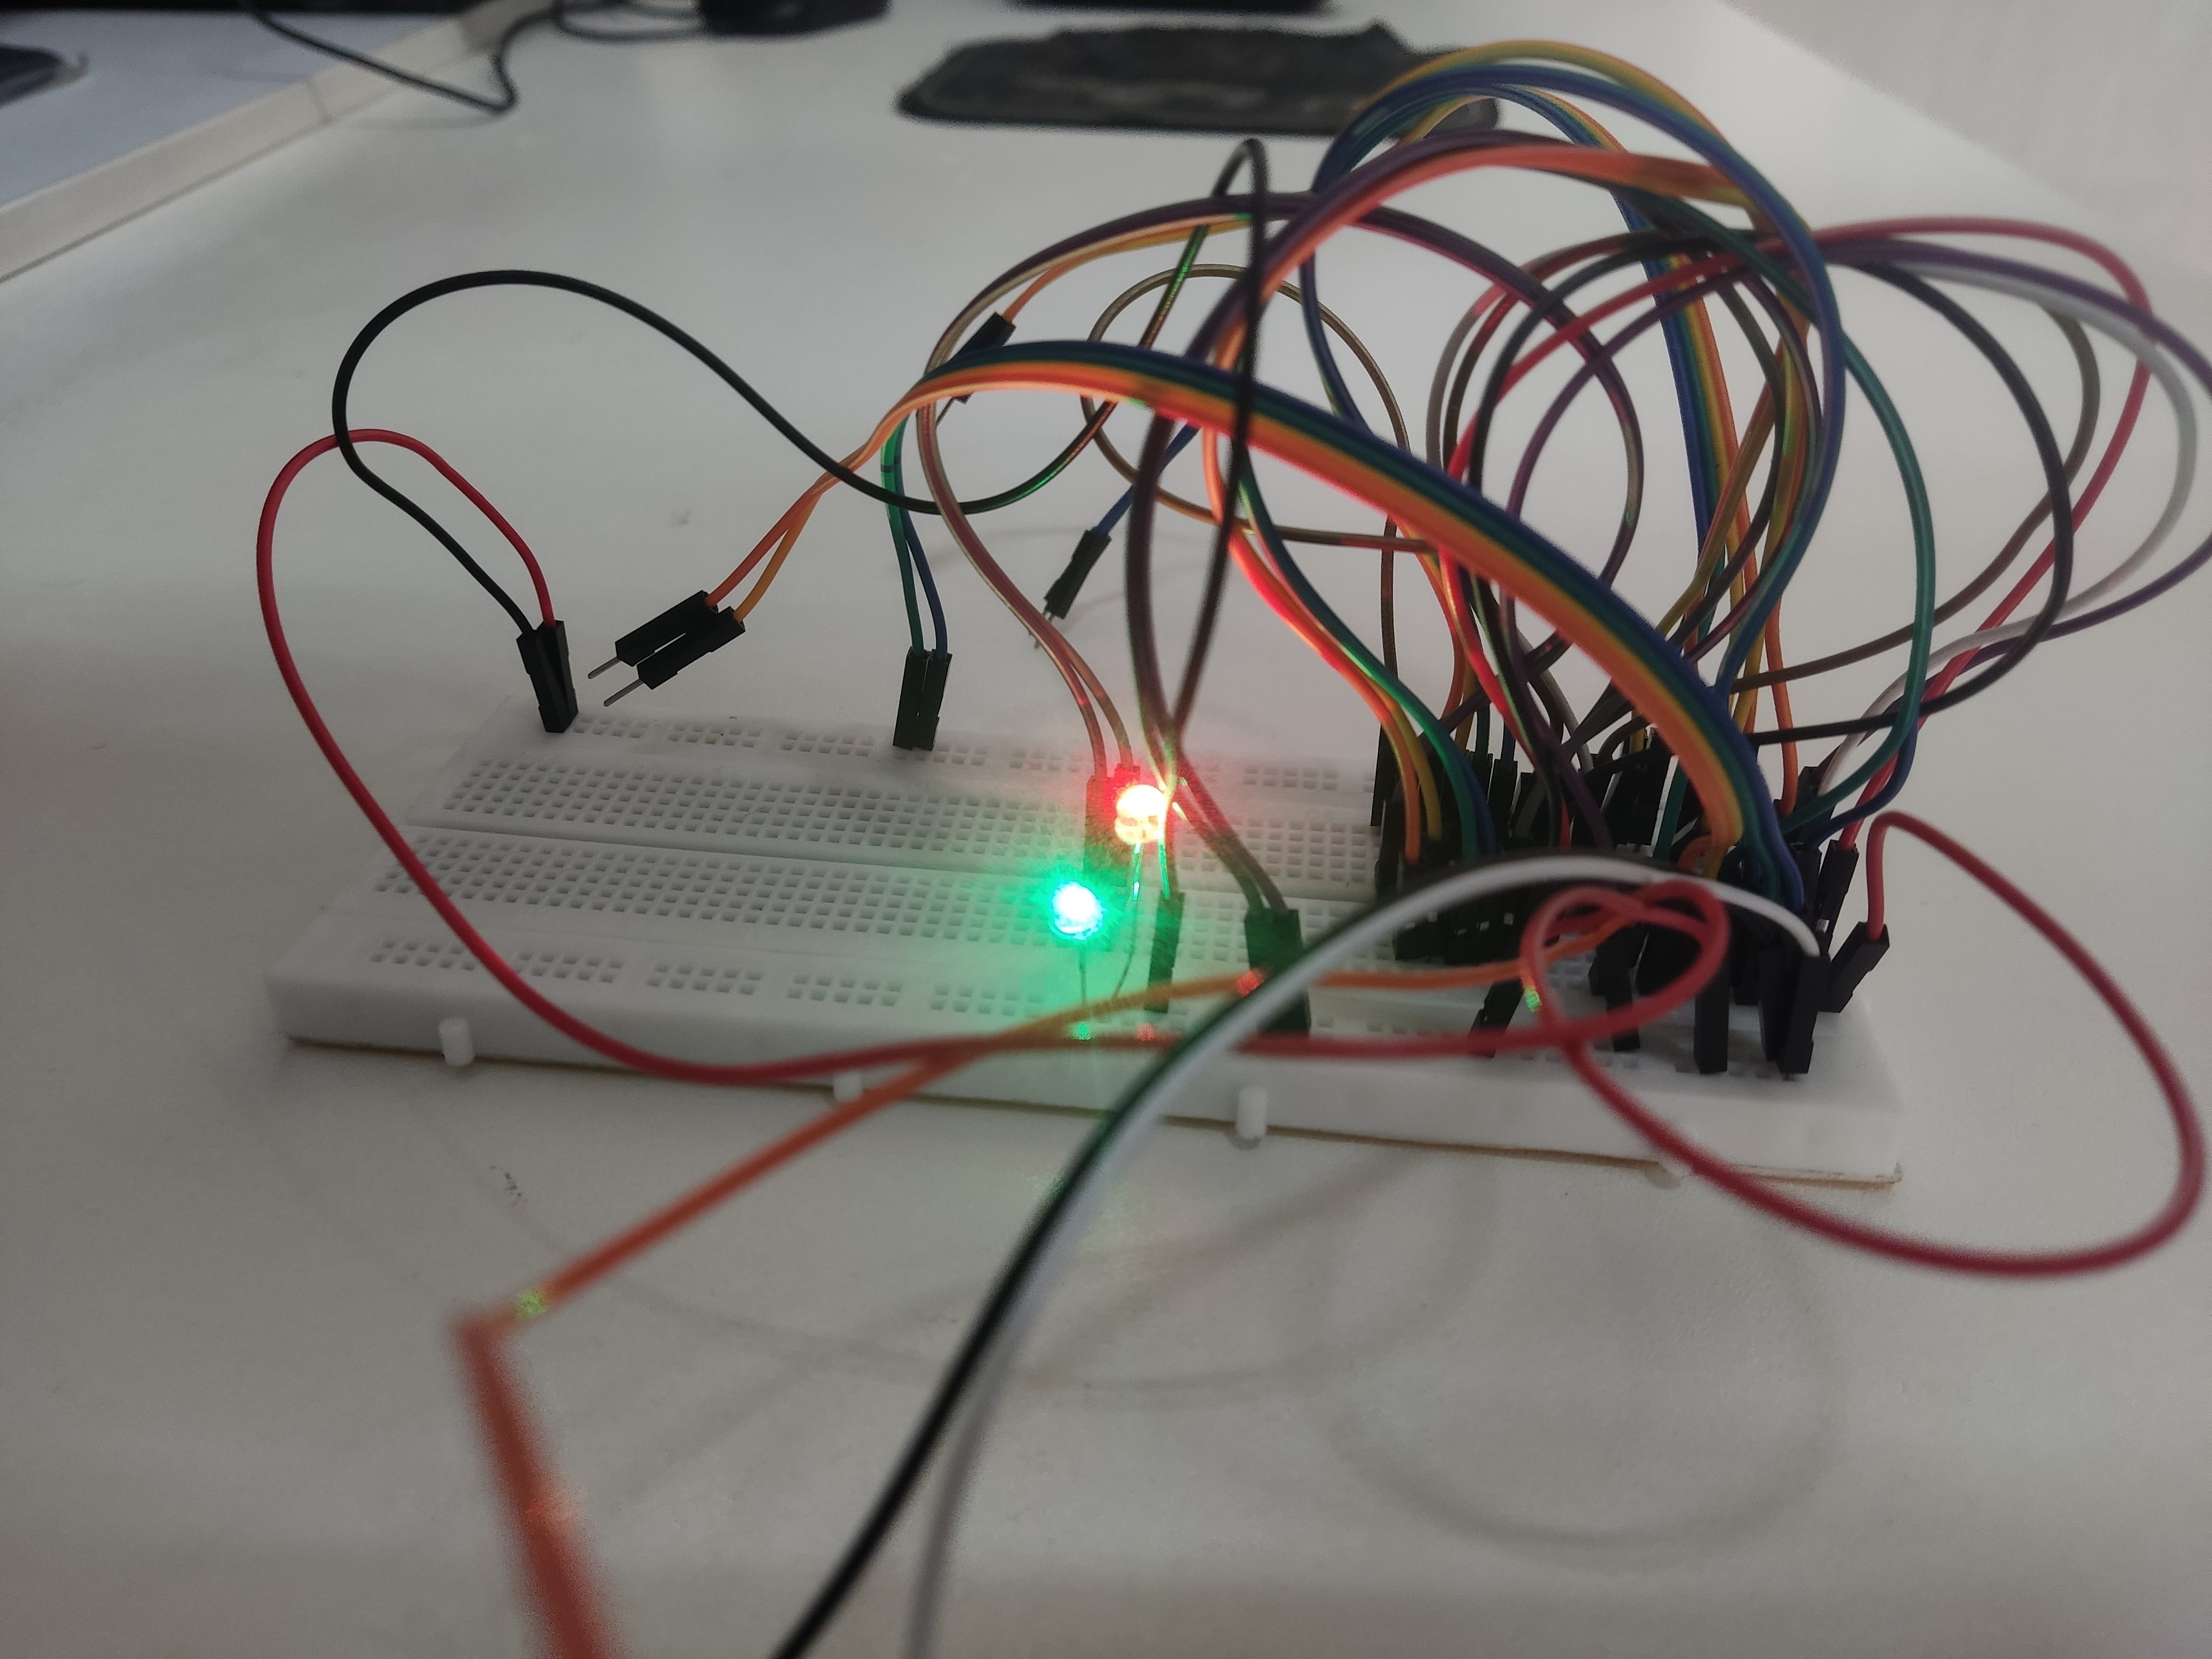
\includegraphics[width=0.85\textwidth]{images/IMG_experiment-result1.jpg}
    \caption{نتیجه آزمایش عملی به ازای \engr{\textbf{S\textsubscript{1}S\textsubscript{0}} = 01}}
    \label{fig:result1}
\end{figure}

\begin{figure}[H]
    \centering
    \includegraphics[width=0.85\textwidth]{images/IMG_experiment-result2.jpg}
    \caption{نتیجه آزمایش عملی به ازای \engr{\textbf{S\textsubscript{1}S\textsubscript{0}} = 11}}
    \label{fig:result2}
\end{figure}

\end{document}
